% ========================================================================================================
% Introduction 

\minitoc 

Dans ce second chapitre, nous allons nous intéresser aux problème d'optimisation avec contraintes. 
Ces problèmes sont plus génériques que ceux vu précédement et demandent l'utilisation de nouveaux 
outils pour les traiter. Voyons-en un exemple. 

\begin{example}
    Reprenons un problème d'optimisation classique, auxquel on rajoute une condition : 
        \begin{mini}|l|
                {}{f(x) = x^2}{}{}
                \addConstraint{x}{ \geqslant 1}
                \addConstraint{x}{\in \mathcal{\R}}
        \end{mini}
    
    La solution évidente de ce problème est bien $x = 1$. Or la première condition nécessaire d'optimalité 
    vue précédement n'est plus valable. En effet, $f'(1) = 1 \not = 0$. 
    Nous devons donc en définir de nouvelles.
\end{example}

Soient $f : \R^n \longrightarrow \R$ et $C \subseteq \R^n$.
Dans ce chapitre, nous traiterons donc des problèmes nommés $ (\mathcal{P})$ de la forme :

    \begin{mini*}|l|
        {}{f(x)}{}{}
        \addConstraint{x}{ \in C}
    \end{mini*}

L'objectif de ce chapitre est de donc de définir une nouvelle notion de point critiques pour les 
problèmes d'optimisation avec contrainte mais aussi de donner des critères d'optimalité. 
La seconde partie de ce chapitre sera consacrée à la présentation d'algorithmes itératifs de 
recherche de solutions. 

% ========================================================================================================
% Optimisation sous contraintes : Approche géométrique 

\section{Optimisation sous contraintes : Approche géométrique}
Dans cette section, nous allons explorer les problèmes d'optimisation avec contraintes à travers une approche géométrique. L'objectif est de comprendre intuitivement pourquoi les solutions optimales se trouvent à des endroits spécifiques.

\subsection{Contraintes d'égalité}
Considérons un problème simple avec une contrainte d'égalité :
\begin{example}
    Minimiser \( f(x, y) = x^2 + y^2 \) sous la contrainte \( x + y = 1 \).

    \begin{center}
        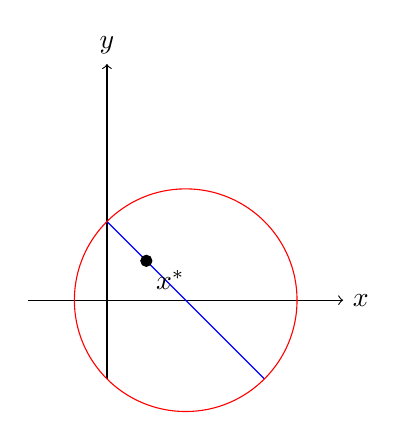
\begin{tikzpicture}[scale=1.0]
            \draw[->] (-1,0) -- (3,0) node[right]{$x$};
            \draw[->] (0,-1) -- (0,3) node[above]{$y$};
            \draw[domain=0:2, smooth, variable=\x, blue] plot ({\x}, {1 - \x});
            \draw[red] (1,0) circle (1.414);
            \filldraw[black] (0.5,0.5) circle (2pt) node[anchor=north west]{$x^*$};
        \end{tikzpicture}
    \end{center}

    La solution optimale \( x^* = (0.5, 0.5) \) est le point où la courbe de niveau de \( f \) est tangente à la contrainte.
\end{example}

\subsection{Contraintes d'inégalité}

Passons maintenant à un problème avec une contrainte d'inégalité :

\begin{example}
    Minimiser \( f(x, y) = x^2 + y^2 \) sous la contrainte \( x + y \geq 1 \).

    \begin{center}
        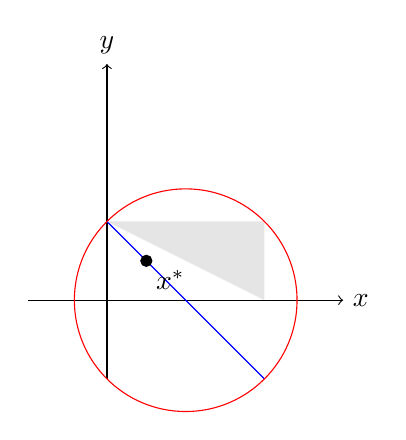
\begin{tikzpicture}[scale=1.0]
            \draw[->] (-1,0) -- (3,0) node[right]{$x$};
            \draw[->] (0,-1) -- (0,3) node[above]{$y$};
            \draw[domain=0:2, smooth, variable=\x, blue] plot ({\x}, {1 - \x});
            \fill[gray!20] (0,1) -- (2,1) -- (2,0) -- cycle;
            \draw[red] (1,0) circle (1.414);
            \filldraw[black] (0.5,0.5) circle (2pt) node[anchor=north west]{$x^*$};
        \end{tikzpicture}
    \end{center}

    La solution optimale \( x^* = (0.5, 0.5) \) se trouve sur la frontière de la contrainte.
\end{example}

% ========================================================================================================
% Conditions d'optimalité : Construction pas à pas

\section{Conditions d'optimalité : Construction pas à pas}
Nous allons maintenant formaliser les conditions d'optimalité pour les problèmes avec contraintes.

\subsection{Contraintes d'égalité}
\subsubsection{Approche intuitive}
Pour un problème avec contraintes d'égalité, si \( x^* \) est optimal, alors le gradient de \( f \) en \( x^* \) doit être orthogonal à l'espace tangent des contraintes. Cela signifie que :
\[
\nabla f(x^*) + \sum_{j=1}^m \lambda_j \nabla h_j(x^*) = 0
\]
où \( \lambda_j \) sont les multiplicateurs de Lagrange.

\subsubsection{Théorème de Lagrange}
\begin{theorem}
    Soit \( f : \R^n \to \R \) et \( h : \R^n \to \R^m \) des fonctions différentiables. Si \( x^* \) est un minimum local de \( f \) sous les contraintes \( h(x) = 0 \), alors il existe \( \lambda \in \R^m \) tel que :
    \[
    \nabla f(x^*) + \sum_{j=1}^m \lambda_j \nabla h_j(x^*) = 0.
    \]
\end{theorem}

\begin{example}
    Reprenons l'exemple \( f(x, y) = x^2 + y^2 \) sous \( x + y = 1 \). Le lagrangien est :
    \[
    L(x, y, \lambda) = x^2 + y^2 + \lambda (1 - x - y).
    \]
    Les conditions d'optimalité donnent :
    \[
    2x - \lambda = 0, \quad 2y - \lambda = 0, \quad 1 - x - y = 0.
    \]
    La solution est \( x^* = (0.5, 0.5) \).
\end{example}

\subsection{Contraintes d'inégalité}
\subsubsection{Approche intuitive}
Pour les contraintes d'inégalité, si une contrainte est inactive (\( g_i(x) < 0 \)), elle ne joue aucun rôle. Si elle est active (\( g_i(x) = 0 \)), on se ramène au cas d'égalité.

\subsubsection{Conditions KKT}
\begin{theorem}
    Soit \( f : \R^n \to \R \), \( g : \R^n \to \R^p \), et \( h : \R^n \to \R^m \) des fonctions différentiables. Si \( x^* \) est un minimum local de \( f \) sous les contraintes \( g(x) \leq 0 \) et \( h(x) = 0 \), et si une condition de qualification des contraintes (CQ) est satisfaite, alors il existe \( \mu \in \R^p \) et \( \lambda \in \R^m \) tels que :
    \begin{enumerate}[label=\roman*)]
        \item \( \nabla f(x^*) + \sum_{i=1}^p \mu_i \nabla g_i(x^*) + \sum_{j=1}^m \lambda_j \nabla h_j(x^*) = 0 \),
        \item \( \mu_i \geq 0 \) pour tout \( i \),
        \item \( \mu_i g_i(x^*) = 0 \) pour tout \( i \) (complémentarité).
    \end{enumerate}
\end{theorem}

\subsection{Théorème de Fritz John}
\subsubsection{Motivation}
Que se passe-t-il si les hypothèses des conditions KKT ne sont pas satisfaites ? Le théorème de Fritz John fournit une réponse.

\begin{theorem}
    Soit \( x^* \) un minimum local de \( f \) sous les contraintes \( g(x) \leq 0 \) et \( h(x) = 0 \). Alors il existe \( \mu_0 \in \R \), \( \mu \in \R^p \), et \( \lambda \in \R^m \), non tous nuls, tels que :
    \begin{enumerate}[label=\roman*)]
        \item \( \mu_0 \nabla f(x^*) + \sum_{i=1}^p \mu_i \nabla g_i(x^*) + \sum_{j=1}^m \lambda_j \nabla h_j(x^*) = 0 \),
        \item \( \mu_0 \geq 0 \),
        \item \( \mu_i \geq 0 \) pour tout \( i \),
        \item \( \mu_i g_i(x^*) = 0 \) pour tout \( i \).
    \end{enumerate}
\end{theorem}

\begin{example}
    Considérons \( f(x) = x \) sous \( g(x) = x^3 \leq 0 \). En \( x^* = 0 \), le théorème de Fritz John donne \( \mu_0 = 0 \) et \( \mu_1 = 1 \), car \( \nabla g(0) = 0 \).
\end{example}

% % ========================================================================================================
% % Conditions d'optimalité

% \section{Conditions d'optimalité}

% \subsection{CN et CNS}

% Commençons par un analogue at principe de Fermat. 

% \begin{theorem}[CN d'optimalité du second ordre]
%     Soit $f : \R^n \longrightarrow \R$ une application et $C \subset \R^n$ \emph{convexe}.
%     Alors tout solution $ \overline{x} \in C$ de $ ( \mathcal{P})$ safisfait la condition nécessaire 
%     d'optimalité du second ordre : 
%         \begin{equation}
%             \forall x \in C, \quad \langle \nabla f( \overline{x}), \overline{x} - x \rangle \geqslant 0 
%         \end{equation}
% \end{theorem}

% Dans le cas particulier où $C$ et $f$ sont convexes, cette condition nécessaire est aussi suffisante. 

% \begin{theorem}[CNS d'optimalité du second ordre]
%     Soit $f : \R^n \longrightarrow \R$ une fonction convexe différentiable et $C \subset \R^n$ convexe. 
%     Alors $ \overline{x} \in C$ est une solution de $( \mathcal{P})$ ssi : 
%         \begin{equation}
%             \forall x \in C, \quad \langle \nabla f( \overline{x}), \overline{x} - x \rangle \geqslant 0 
%         \end{equation}
% \end{theorem}

% \subsection{Optimalité non qualifiée}

% Attardons nous maintenant sur les problèmes d'optimisation $(\mathcal{P})$ de la forme suivante : 

%     \begin{mini*}|l|
%         {}{f(x)}
%         \addConstraint{g(x)}{ \leqslant 0}
%         \addConstraint{f(x)}{ = 0}
%     \end{mini*}

% où $f : \R^n \longrightarrow \R$, $ h : \R^n \longrightarrow \R^m$ et $ g : \R^n \longrightarrow \R^p$.


% \begin{theorem}[F. John, 1948]
%     Soient $f,g,h \in \mathcal{C}^2(\R^n)$. Soit $ \overline{x}$ une solution de $ (\mathcal{P})$.
%     Il existe alors $ \mu_0 \in \R$ et $ \mu \in \R^p$, $ \lambda \in \R^m$ vérifiants des conditions 
%     dites \emph{non qualifiées} suivantes :
%         \begin{enumerate}[label=\roman*)]
%             \item $ \mu_0 \nabla f( \overline{x}) + \displaystyle\sum_{i=1}^{p} \mu_i \nabla g_i( \overline{x}) + \sum_{j=1}^{m} \lambda_i \nabla h_i( \overline{x}) = 0 $
%             \item $ \mu_0 \geqslant 0 $ 
%             \item $ \forall i \in \llbracket 1, p \rrbracket, \quad \mu_i \geqslant 0 $
%             \item $ \forall i \in \llbracket 1, p \rrbracket, \quad \mu_i g_i( \overline{x}) = 0 $
%         \end{enumerate}
% \end{theorem}

% \begin{remark}
%     \begin{itemize}
%         \item Les réels $ \lambda_i $ et $ \mu_i$ sont appelés \emph{multiplicateurs de Lagrange} du problème. 
%         \item Un vecteur $x \in \R^n$ est dit \emph{réalisable} ou \emph{admissible} pour $ ( \mathcal{P})$ s'il 
%         satisfait les contraintes $ g(x) \leqslant 0$ et $h(x) = 0$.
%         \item La condition iv) est appelée \emph{complémentarité}.
%     \end{itemize}
% \end{remark}

% \subsection{Qualification des contraintes}

% Une contrainte d'inégalité $ g(x) \leqslant 0$ est dite \emph{active} $y \in \R^n$ si $g(y) = 0$. 
% On note $ \mathcal{J}(x)$ l'ensemble des indices des contraintes actives en $x$ : 
%     $$ \mathcal{J}(x) := \{i \in \llbracket 1, p \rrbracket \mid g_i(x) = 0\} $$ 

% \begin{definition}[Conditions de qualification de Mangasarian-Fromovitz]
%     Un vecteur $ y \in \R^n$ satisfait les conditions de qualification de Mangasarian-Fromovitz (MF) pour 
%     le problème $( \mathcal{P})$ si : 
%     \begin{enumerate}[label=\roman*)]
%         \item $x$ est \emph{admissible} en $ h(x) = 0$ et $g(x) = 0$. 
%         \item les $m$ vecteurs $ \nabla h_i(x)$ sont \emph{linéairement indépendants}.
%         \item il existe $d \in \R^n / \{0\}$ tel que : 
%             \begin{equation}
%                 \forall j \in \llbracket 1, m \rrbracket \quad \langle \nabla h_j(x), d \rangle = 0 
%             \end{equation}
%             et : 
%             \begin{equation}
%                 \forall k \in \mathcal{J}(x), \quad \langle \nabla g_k(x),d \rangle = < 0 
%             \end{equation}
%     \end{enumerate}
% \end{definition}

% \begin{definition}[Conditions de qualification 2]
%     On dit que $x \in \R^n$ satisfait les conditions de qualifications (CQ2) pour les contraintes 
%     correspondant à $g$ et $h$ si : 
%     \begin{enumerate}[label=\roman*)]
%         \item $x$ esr admissible.
%         \item la famille de vecteurs : 
%             \begin{equation}
%                 \{ \nabla h_j(x) \mid j \in \llbracket 1, m \rrbracket\} \cup \{ \nabla g_k(x) \mid k \in \mathcal{J}(x)\}
%             \end{equation}
%             est linéairement indépendante.
%     \end{enumerate}
% \end{definition}

% \begin{proposition}
%     Dans le contexte actuel, un vecteur vérifiant CQ2 verifie aussi MF. D'où $ \text{CQ2} \Longrightarrow \text{MF}$.
% \end{proposition}

% \begin{theorem}[Karush-Kuhn-Tucker]
%     Soient $f,g,h \in \mathcal{C}^2(\R^n)$. Soit $ \overline{x} \in \R^n$ une solution de notre problème. 
%     Si $overline{x}$ satsifait MF, alors il existe $ \mu \in \R^p$ et $ \lambda \in \R^m$ tels que : 
%         \begin{enumerate}[label=\roman*)]
%             \item $ \mu_0 \nabla f( \overline{x}) + \displaystyle\sum_{i=1}^{p} \mu_i \nabla g_i( \overline{x}) + \sum_{j=1}^{m} \lambda_i \nabla h_i( \overline{x}) = 0 $
%             \item $ \forall i \in \llbracket 1, p \rrbracket, \quad \mu_i \geqslant 0 $
%             \item $ \forall i \in \llbracket 1, p \rrbracket, \quad \mu_i g_i( \overline{x}) = 0 $
%         \end{enumerate}
% \end{theorem}

% \begin{definition}[Lagrangien]
%     Le lagrangien du problème $( \mathcal{P})$ est la fonction définie sur $ \R^n \times \R^p \times \R^m$ par : 
%         \begin{align}
%             L(x, \mu, \lambda) &= f(x) + \sum_{i=1}^{p} \mu_i g_i(x) \sum_{i=1}^{m} \lambda_i h_i(x) \\ 
%             &= f(x) + \langle \mu, g(x) \rangle + \langle \lambda, h(x) \rangle
%         \end{align}
% \end{definition}

% \subsection{Suffisance dans le cas convexe}



